\section{Methods}
\subsection{Participants}
\subsection{Design}
This study explored the impact of various gamified elements and participant gender on performance and anxiety.
The independent variables were gamified elements, with participants randomly assigned to one of eight conditions: Avatars (A), Badges (B), Points (P), Leaderboards (L), Narrated Content (N), combinations of Points, Badges, Leaderboards, and Avatars (PBLA), Points, Badges, Leaderboards, Avatars, and Narrated Content (PBLAN), and a control group with no gamified elements.
Each participant experienced three distinct conditions, which were sent by the server out of a randomized pregenerated batch, ensuring that all conditions were evenly distributed across participants.
Participants underwent a series of tests in a fixed order during each round, beginning with a gamified performance test in a digital learning environment followed by  not gamified assessments for anxiety, self-efficacy, and motivation.
At the end participants were given a monetary compensation of 15€.
The performance tests utilized standard progressive matrices, adapted with gamification techniques to engage and challenge participants uniquely in each round.
The dependent variables included:
\begin{itemize}
  \item \textbf{Performance}, assessed through accuracy and response times in the gamified progressive matrices.
  \item \textbf{Anxiety}, evaluated using a standardized questionnaire immediately after the performance test. Anxiety was measured using a shortened form of the State-Trait Anxiety Inventory (STAI) with 6 items \parencite{marteauDevelopmentSixitemShortform1992}.
\end{itemize}

Although self-efficacy and motivation were also assessed \parencite{chenValidationNewGeneral2001,guayAssessmentSituationalIntrinsic2000} through subsequent questionnaires, these variables were not analyzed within the scope of this bachelor thesis.
The collected data for self-efficacy and motivation are intended for use in the doctoral dissertation of \textbf{Nadine Koch}.
This research employed a repeated-measures design, where each participant was exposed to three different gamification conditions chosen randomly.
This within-subjects approach facilitated the analysis of individual responses to each condition across the different rounds, providing insights into how variations in gamification can affect psychological states and performance.
The sequence and consistency of the testing procedure, including the series of questions asked in the gamified digital learning environment were always maintained to ensure the reliability of measurements and comparability of results across the various stages of the experiment.


\subsection{Materials}
\subsubsection{Physical environment}
The study was conducted in two separate rooms in the cellar of a university building, one equipped with five and one with seven iMacs.
As \textcite{christyLeaderboardsVirtualClassroom2014} suggested that the physical environment can influence the results, so both rooms are equipped with the same furniture and lighting and are furnished very dry, like a typical software laboratory.

\subsection{Virtual environment}
The software used in this study was build by the author using SvelteKit in frontend and Ktor in backend. Its UI is designed after the study by \textcite{albuquerqueDoesGenderStereotype2017}.
On the iMac's the study was displayed full-screen mode using the Safari web browser to ensure no further distractions. The study consisted of 4 screens.
A consent screen to give an overview and explain the data collection to the user.
A personal detail screen to collect said data; gender, age and study program. Participants also had to enter a deletion code in order to request their data's deletion after the collection.
\begin{figure}[H]
  \centering
  \includegraphics[width=0.5\textwidth]{img/details.png}
  \caption{The personal details collection form}
  \label{fig:figureDetails}
\end{figure}
The next screen was the gamified learning environment, where the participants had to solve 20 questions in a row while being exposed to the gamified elements.
The matrices were taken from \textcite{albuquerqueDoesGenderStereotype2017}, to generate 60 questions out of the 20, the 40 questions for iteration two and three were slightly altered versions of the original 20 made by this author.
\begin{figure}[H]
  \centering
  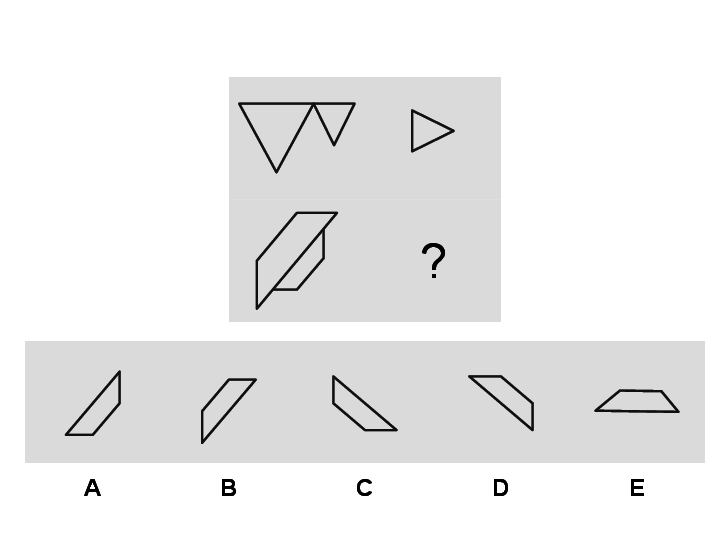
\includegraphics[width=0.5\textwidth]{img/q-17.png}
  \caption{A standard progressive matrix, one of the tasks given to the participants}
  \label{fig:figureMatrix}
\end{figure}
The gamified learning environment consists of different UI elements representing the gamified elements.
\begin{description}
  \item[Leaderboards]: A list of participants and scores, including the current participant. The other players shown are not real.
  \item[Badges]: An array of four badges that are awarded for 1, 5, 10 and 18 correctly answered questions.
  \item[Avatars]: A small avatar that is shown in the top right corner of the screen and on the leaderboard. To increase identification with the avatar further, the participants were asked to choose one of 15 different avatars before the iteration.
  \item[Narrated content]: Narrated content is shown in the bottom right corner of the screen. It is presented as a speech bubble with an avatar next to it, in case avatars are enabled. It shows a random praise or encouragement sentence every three questions.
  \item[Points]: A counter next to the question frame shows the current points. One point is awarded for each correctly answered question. THe narrated content is shown every three questions.
\end{description}
After answering one question the next question has a one-second delay which increases to four seconds if narrated content is shown.
\begin{figure}[H]
  \centering
  \begin{subfigure}[t]{0.4\textwidth}
    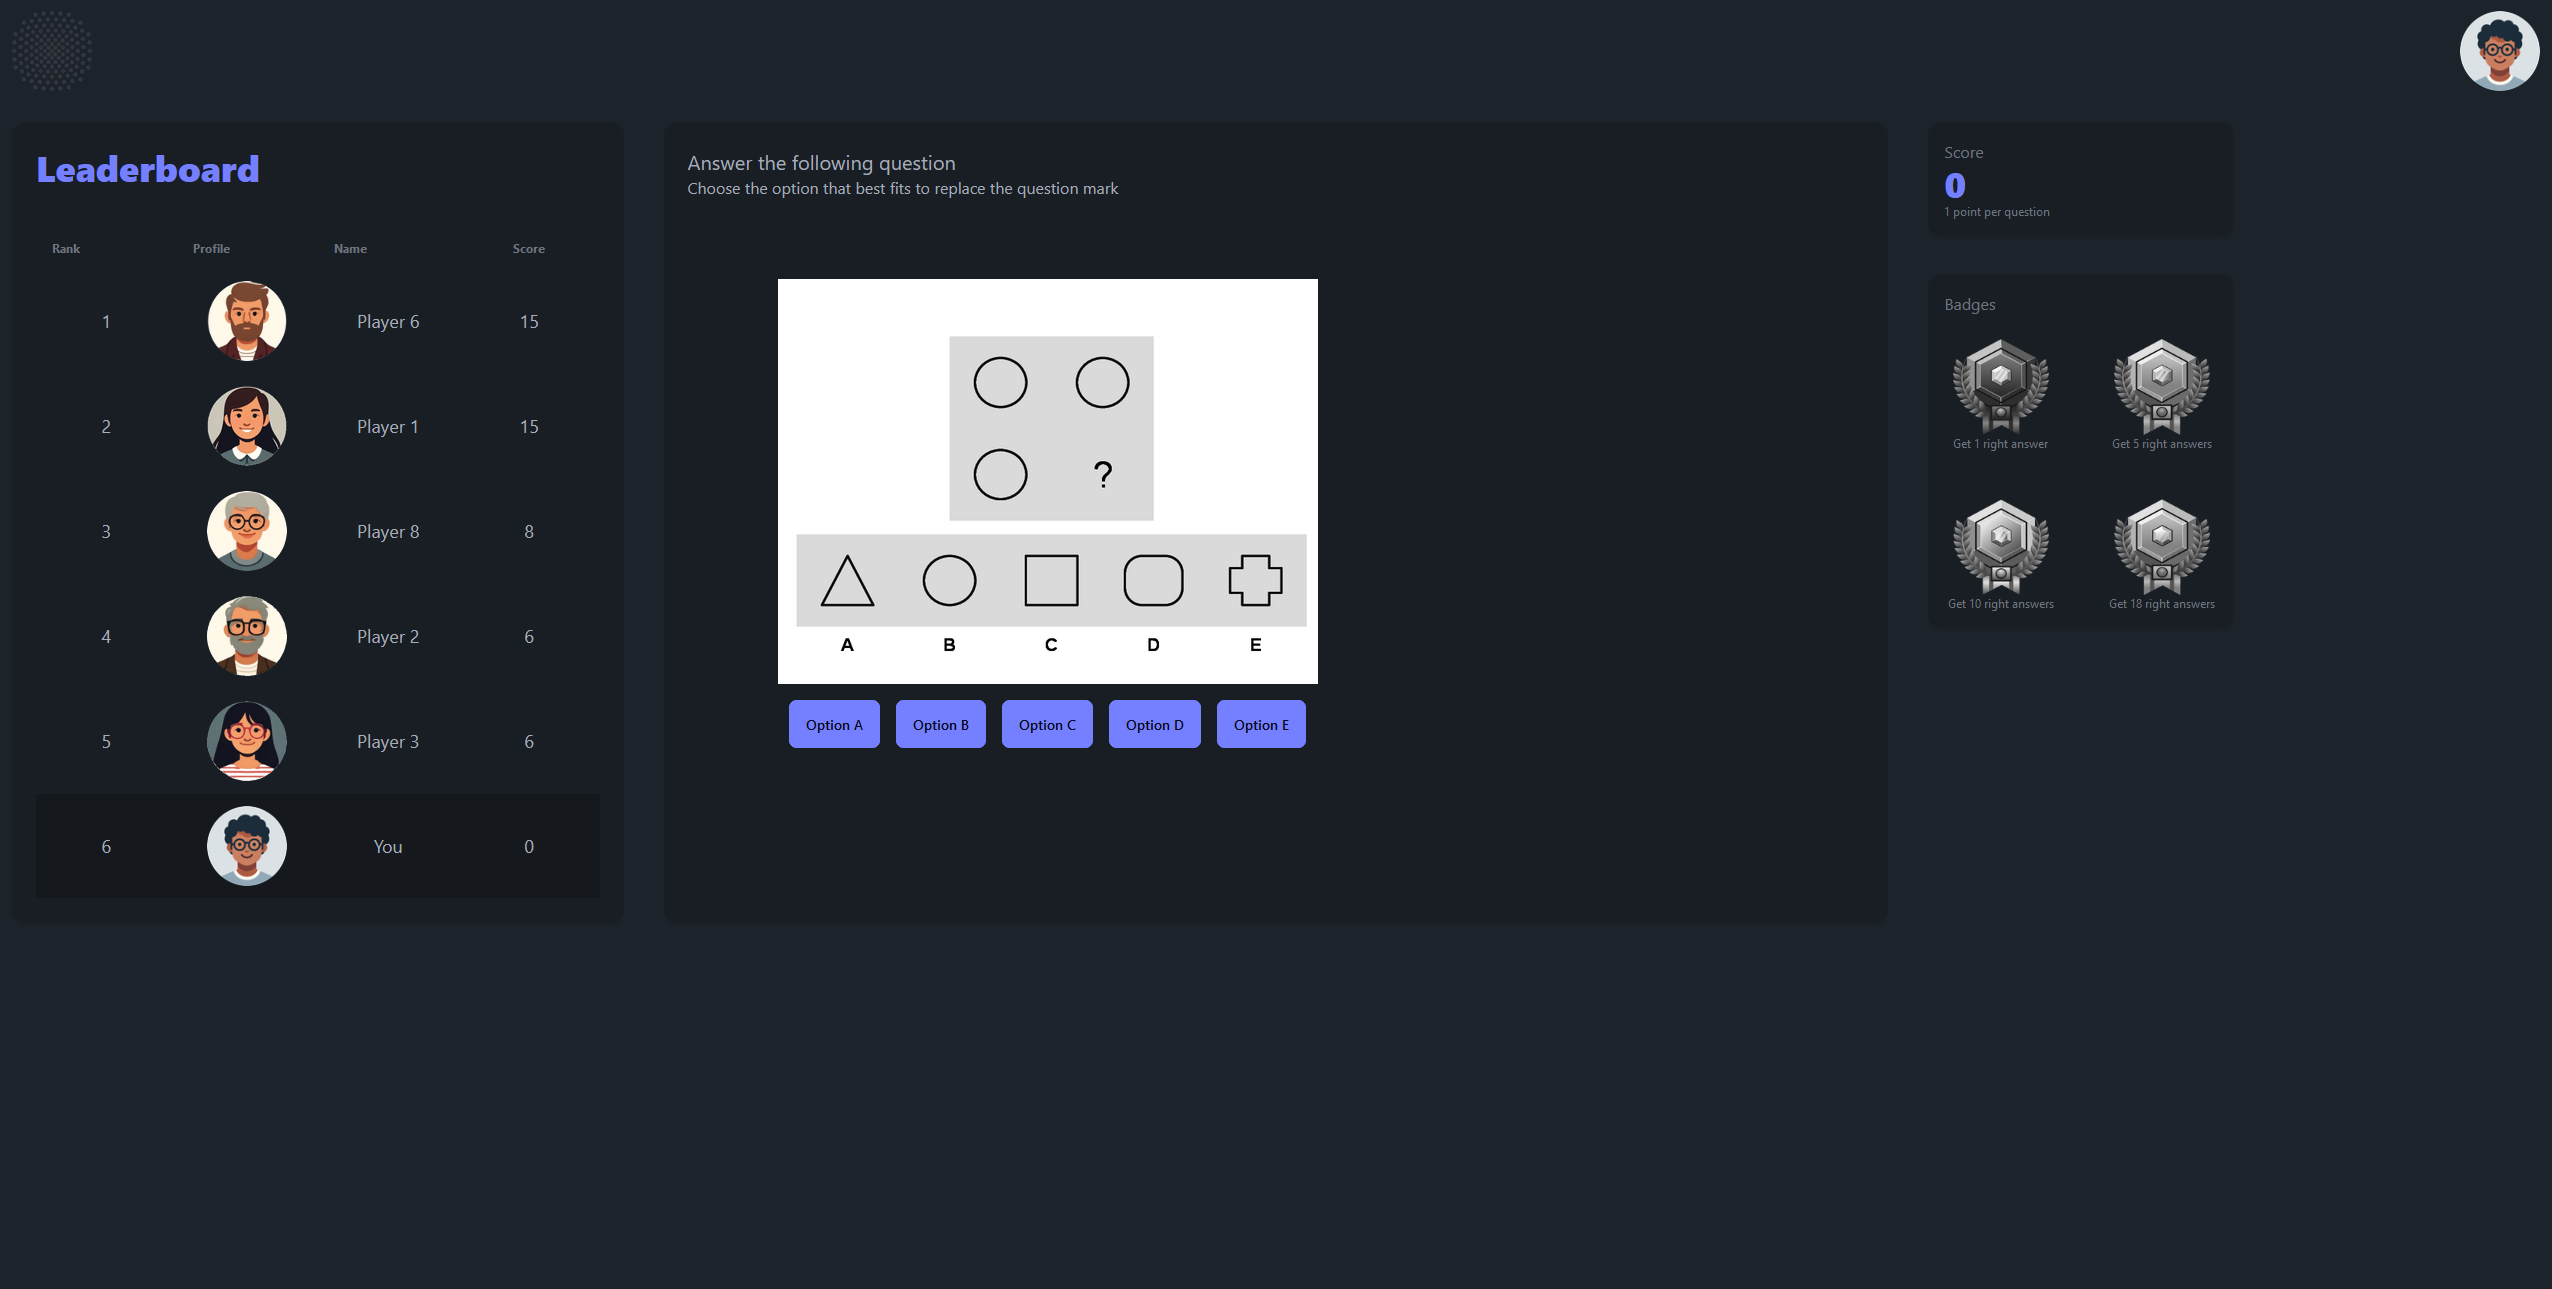
\includegraphics[width=\textwidth]{img/question_screen.png}
    \caption{The Digital Learning Environment with Points, Badges, Leaderboards and Avatars enabled}
    \label{fig:figureScreenEnabled}
  \end{subfigure}
  \hspace{5mm}
  \begin{subfigure}[t]{0.4\textwidth}
    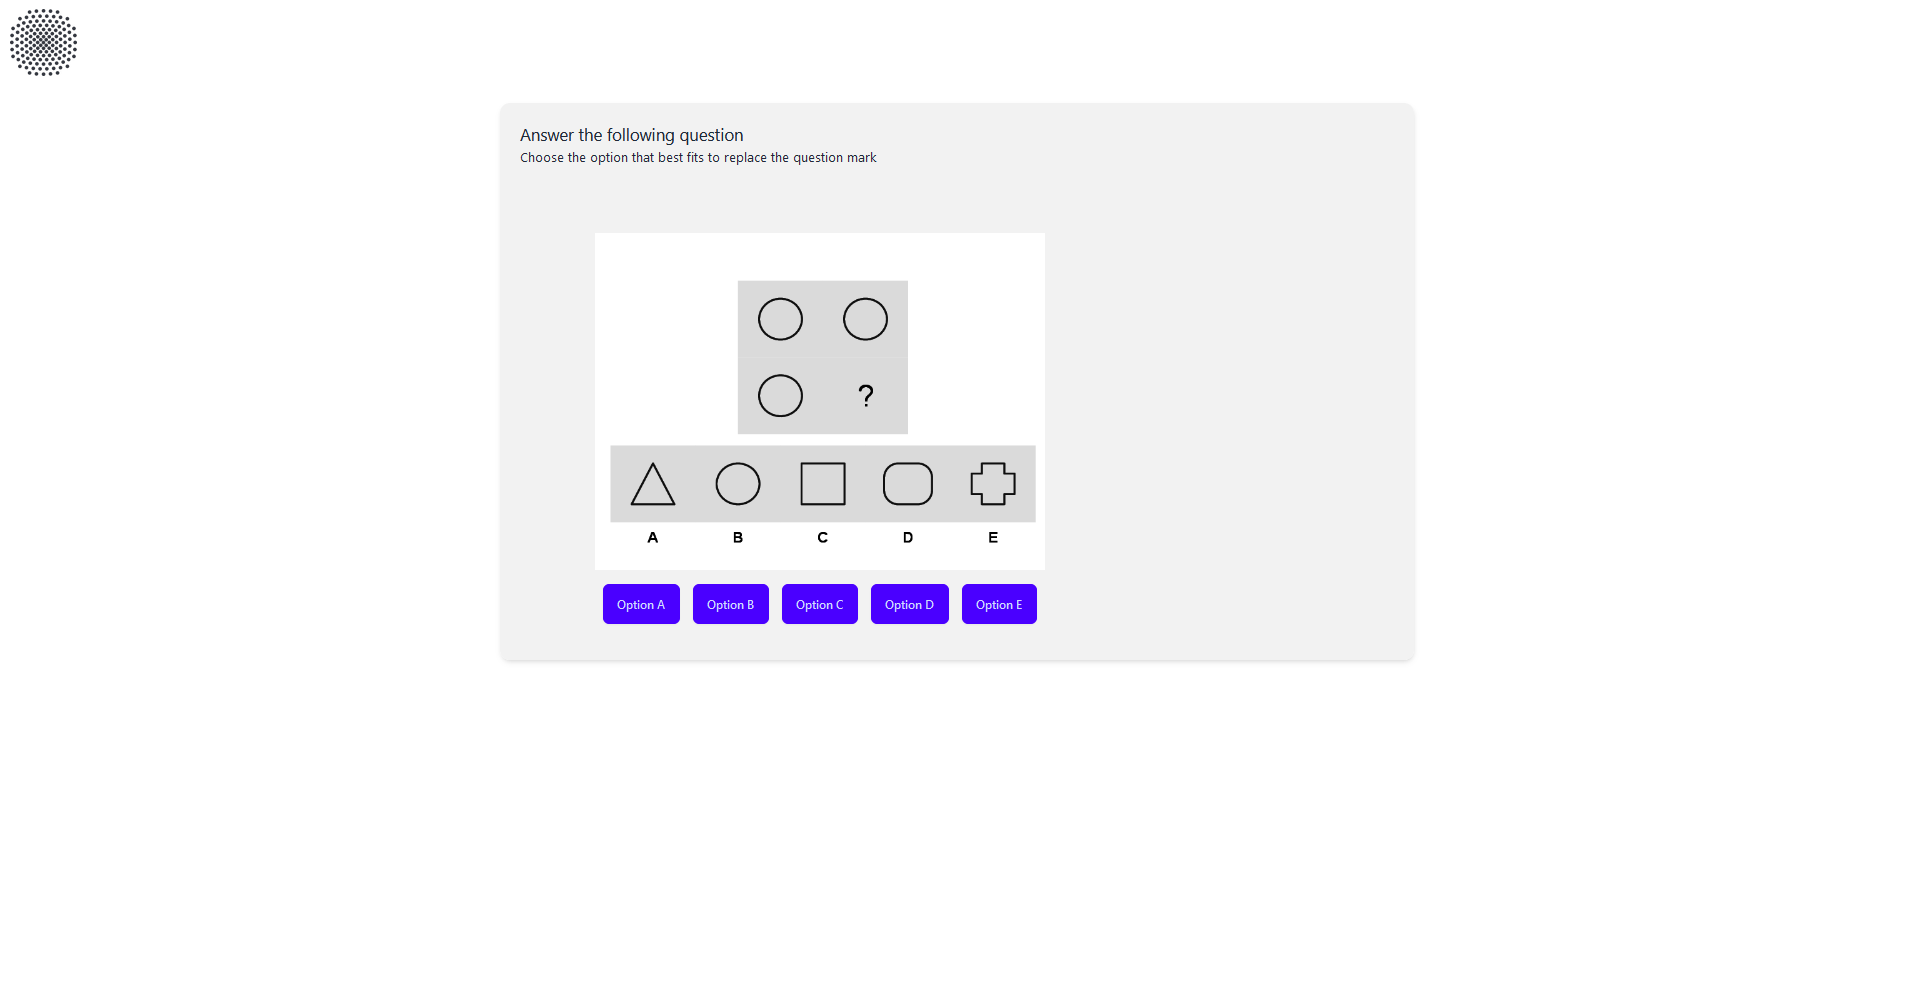
\includegraphics[width=\textwidth]{img/question_screen_no_elements.png}
    \caption{The Digital Learning Environment with no Gamified Elements enabled}
    \label{fig:figureScreenDisabled}
  \end{subfigure}
  \caption{Comparison of the Digital Learning Environment with and without gamified elements enabled}
\end{figure}

After the gamified learning environment, the participants were shown a questionnaire for anxiety, motivation and self-efficacy. The three questionnaires were a six-question shortened form of the State-Trait Anxiety Inventory (STAI) \parencite{marteauDevelopmentSixitemShortform1992}, the eight-question General Self-Efficacy Scale (GSE) \parencite{guayAssessmentSituationalIntrinsic2000} and the 16-question Situational Intrinsic Motivation Scale (SIMS) \parencite{chenValidationNewGeneral2001}.

\subsection{Scoring}
Scoring was done in R manually. The data was cleaned up before the analysis.
The scores for the different conditions were calculated as follows:
\begin{description}
  \item[Performance] was calculated as the sum of the correctly answered questions divided by all questions. If this value was below 0.25 the particular dataset was excluded from the analysis.
  \item[STAI] was calculated using the formula provided by \textcite{marteauDevelopmentSixitemShortform1992}. As participants had answers from "Not at all" to "Very much so" the answers are represented by numbers from zero to five. As the original test has 20 questions, weights according to \textcite{marteauDevelopmentSixitemShortform1992} were applied to the answers. Negative weights were applied for negative questions like "Right now I am worried".
  \item[New GSE] was calculated using the formula provided by \textcite{guayAssessmentSituationalIntrinsic2000}. The mean of the number representation of the answers was calculated.
  \item[] 
\end{description}